\begin{center}
  \textsf{Листок 7.}
\end{center}
\vspace{0.01mm}
\nopagebreak[2]

\taskpic{ 
Два одинаковых кубика с длиной ребра $b$ массой $m$ каждый
  стоят на горизонтальном столе, на расстоянии $b$ друг от друга. Между
  ними помещён рычаг длиной $2^{3/2}b$ с пренебрежимо малой
  массой. Коэффициент трения между поверхностями кубиков и столом
  $k$. Коэффициент трения между рычагом и кубиками очень большой в точке
  $A$ и очень маленький в точке $C$. В точке $B$ приложена сила $F$,
  направленная перпендикулярно рычагу как показано на
  рисунке. Определите, какой из кубиков сдвигается раньше, если
  постепенно увеличивать силу $F$.  }
{ 
\begin{tikzpicture}[interface/.style={postaction={draw,decorate,decoration={border,angle=-45,amplitude=0.2cm,segment
        length=1.5mm}}},>=latex]
    \draw[interface] (0.2,0) -- (3.6,0);
    \draw[thick] (0.4,0) rectangle ++(1,1) node[midway]
    {$m$} ++(1,-1) rectangle ++(1,1) node[midway] {$m$};
    \coordinate (a) at (1.4,0);
    \coordinate (f) at ($(a)!2!(2.4,1)$);
    \draw[thick] (a) -- (f);
    \draw[->] (f) -- ++(-45:1) node[below] {$\vec{F}$};
  \end{tikzpicture}
%\includegraphics[width=4cm]{p09_26.pdf}
}

\taskpic{ Однородный стрежень длиной $l$ опирается о пол и
  ступеньку. Коэффициент трения между стержнем и полом равен 1, трения
  между стержнем и ступенькой нет. При какой высоте ступеньки стержень
  может находиться в равновесии, если угол $\alpha = \pi /4$?
}{
  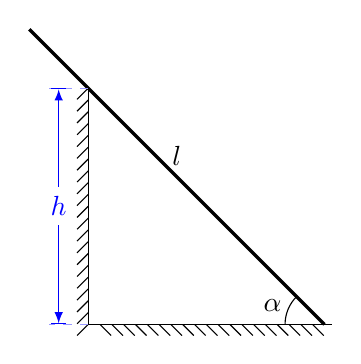
\begin{tikzpicture}[interface/.style={postaction={draw,decorate,decoration={border,angle=-45,amplitude=0.2cm,segment length=1.5mm}}},>=latex]
    \draw[interface] (0,3) -- (0,0) -- (3.1,0);
    \draw[very thick] (3,0) -- +(135:5.3) node[midway, above] {$l$};
    \draw (3,0) +(135:0.5) arc (135:180:0.5);
    \path (3,0) + (160:0.7) node{$\alpha$};
    \draw[dashed,blue!40] (0,0) -- +(-0.5,0) node [coordinate, near end] (a) {};
    \draw[dashed,blue!40] (0,3) -- +(-0.5,0) node [coordinate, near end] (b) {};
    \draw[blue,|<->|] (a) -- node[fill=white] {$h$} (b);
  \end{tikzpicture}
% \includegraphics[width=4cm]{p09_27.pdf}
}

\taskpic{ В системе, изображённой на рисунке, трение в блоках и между
  другими поверхностями отсутствует. Если грузу массой $m$ позволить
  двигаться, то за какое время он достигает подставки? Начальная
  скорость груза равна нулю, начальное расстояние от груза до
  подставки $h$, нить невесомая и нерастяжимая. Масса подставки $M$.
}{
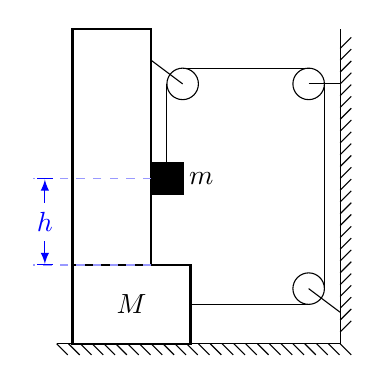
\begin{tikzpicture}[interface/.style={postaction={draw,decorate,decoration={border,angle=-45,amplitude=0.2cm,segment length=1.5mm}}},>=latex]
  \draw[interface] (0.2,0) -- ++(3.6,0) -- ++ (0,4);
  \draw[thick] (0.4,0) rectangle ++(1.5,1) node[midway] {$M$};
  \draw[thick] (0.4,1) rectangle ++(1,3);
  \draw (1.9,0.5) -- (3.4,0.5);
  \filldraw[white,draw=black] (3.4,0.7) circle (0.2);
  \draw (3.4,0.7) -- ++(0.4,-0.3);
  \draw (3.6,0.7) -- ++(0,2.6);
  \filldraw[white,draw=black] (3.4,3.3) circle (0.2);
  \draw (3.4,3.3) -- ++(0.4,0);
  \draw (3.4,3.5) -- ++(-1.6,0);
  \filldraw[white,draw=black] (1.8,3.3) circle (0.2);
  \draw (1.8,3.3) -- ++(-0.4,0.3);
  \draw (1.6,3.3) -- ++(0,-1);
  \draw[fill=black,thick] (1.4,2.3) rectangle ++(0.4,-0.4) node[midway,right=0.15cm]
  {$m$};
  \draw[dashed,blue!40] (1.4,1) -- +(-1.5,0) node [coordinate, pos=0.9] (a) {};
  \draw[dashed,blue!40] (1.4,2.1) -- +(-1.5,0) node [coordinate, pos=0.9] (b) {};
  \draw[blue,|<->|] (a) -- node[fill=white] {$h$} (b);
  % \draw[dashed] (0,1) -- ++(-0.5,0) ++ (0,2.1) -- ++(1.7,0);
  % \draw[thick,<->] (-0.3,1) -- ++(0,2.1) node[midway,left] {$h$};
\end{tikzpicture}
%\includegraphics[width=4cm]{p09_28.pdf}
}

\taskpic{ Найдите ускорение грузов, если масса каждого груза равна
  $m$. Массами нитей и блоков пренебречь, нити нерастяжимы, трение
  отсутствует.
}{
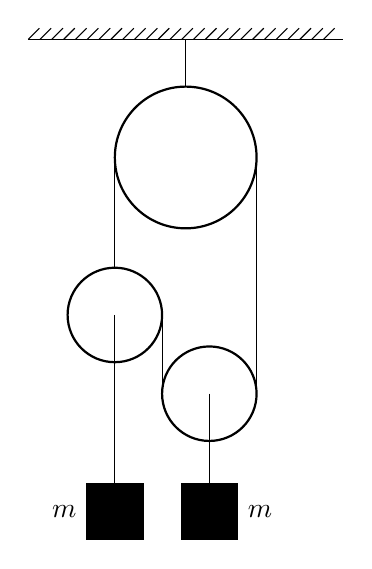
\begin{tikzpicture}[interface/.style={postaction={draw,decorate,decoration={border,angle=45,amplitude=0.2cm,segment length=1.5mm}}},>=latex]
  \draw[interface] (1,0) -- (5,0);
  \draw (3,0) -- (3,-1.5);
  \filldraw[thick,white,draw=black] (3,-1.5) circle (0.9);
  \draw (2.1,-1.5) -- ++(0,-2) (3.9,-1.5) -- ++(0,-3);
  \filldraw[thick,white,draw=black] (2.1,-3.5) circle (0.6);
  \filldraw[thick,white,draw=black] (3.3,-4.5) circle (0.6);
  \draw (2.7,-3.5) -- +(0,-1);
  \draw (2.1,-3.5) -- +(0,-2.5);
  \draw (3.3,-4.5) -- +(0,-1.5);
  \node [rectangle,fill=black,draw=black,thick,label={left:$m$},minimum
  height=0.7cm,minimum width=0.7cm] at (2.1,-6) {};
  \node
  [rectangle,fill=black,draw=black,thick,label={right:$m$},minimum
  height=0.7cm,minimum width=0.7cm] at (3.3,-6) {};
\end{tikzpicture}
%\includegraphics[width=4cm]{p09_29.pdf}
}
